\documentclass[lettersize,journal]{IEEEtran}
\usepackage{amsmath,amsfonts}
\usepackage{algorithmic}
\usepackage{algorithm}
\usepackage{array}
\usepackage[caption=false,font=normalsize,labelfont=sf,textfont=sf]{subfig}
\usepackage{textcomp}
\usepackage{url}
\usepackage{verbatim}
\usepackage{graphicx}
\usepackage{cite}
\usepackage{booktabs}
\usepackage{float}
\usepackage{multirow}

\hyphenation{op-tical net-works semi-conduc-tor IEEE-Xplore}

\begin{document}

\title{Graph-Driven Meta-Agents: Integrating Model Context Protocol and LangGraph for Autonomous Agent Generation}

\author{
Rohan Gamidi\textsuperscript{1},
Tejaswi Muppala\textsuperscript{1},
V. S. S. Ashish Babu\textsuperscript{1},
Vinitha Chowdary A.\textsuperscript{1}, and
S. Santhanalakshmi\textsuperscript{2}
\\
\normalsize
\textsuperscript{1}\{bl.en.u4aie22019, bl.en.u4aie22059, bl.en.u4aie22065, bl.en.u4aie22066\}@bl.students.amrita.edu,
\textsuperscript{2}s\_lakshmi@blr.amrita.edu
\\
\normalsize
\textsuperscript{1,2}Department of Computer Science and Engineering, Amrita School of Computing, Bengaluru, Amrita Vishwa Vidyapeetham, India
}

\markboth{IEEE Transactions on Software Engineering,~Submission}%
{Rohan \MakeLowercase{\textit{et al.}}: Graph-Driven Meta-Agents}

\maketitle

\begin{abstract}
The development of autonomous artificial intelligence agents capable of complex reasoning, tool usage, and workflow orchestration remains a significant challenge in software engineering. Existing frameworks often rely on reactive architectures (e.g., "loops") that require extensive manual configuration and do not natively support planning or workflow refinement. This research proposes a graph-driven "Meta-Agent" architecture that treats agent generation as a compilation process, transforming high-level intent into deterministic executable graphs. The system integrates LangGraph for structured orchestration, the Model Context Protocol (MCP) for standardized tool interoperability, and Retrieval-Augmented Generation (RAG) for grounded reasoning, while employing a novel critic-refiner optimization algorithm that dynamically restructures execution paths based on runtime confidence scores. Experimental evaluation across 240 controlled runs demonstrates that the full system achieves a 91.7\% success rate on complex multi-turn tasks, surpassing reactive baselines such as AutoGPT (48.3\%) and single-LLM approaches (41.7\%). Furthermore, the integration of semantic memory and protocol-driven tooling reduces hallucination rates and improves adaptability. These results indicate that graph-driven meta-agents provide a scalable and reliable foundation for the next generation of autonomous software generation systems.
\end{abstract}

\begin{IEEEkeywords}
Autonomous Agents, LangGraph, Model Context Protocol, Multi-Agent Systems, Retrieval-Augmented Generation, Workflow Orchestration, Adaptive Self-Refinement, Dynamic Graph Optimization.
\end{IEEEkeywords}

\section{Introduction}

\subsection{The Determinism Gap in Autonomous Agents}
\IEEEPARstart{M}{odern} artificial intelligence systems are increasingly required to interact with external APIs, manage state across long horizons, and execute complex workflows. However, the construction of such agents is typically a manual and error-prone process. Developers must explicitly define reasoning loops, tool integration schemas, and memory management logic. A fundamental "determinism gap" exists in current architectures: most deployed agents remain reactive stochastic loops that respond to immediate prompts but lack the capacity to plan extended workflows, refine their own outputs, or generate new sub-agents to handle emerging tasks. This stochasticity results in systems that perform well on single-turn tasks but degrade rapidly in multi-turn engineering scenarios where state consistency is paramount.

\subsection{Agents as Compilation Targets: A Meta-Agent Perspective}
To address these limitations, this research proposes a paradigm shift: viewing agent generation as a compilation process rather than a manual engineering task. In this view, high-level user intent serves as the source code, and the "Meta-Agent" acts as the compiler, transforming this intent into a structured, executable graph of specialized sub-agents. This graph-based control flow ensures that the resulting agent adheres to a defined architectural pattern, enforcing separation of concerns between reasoning, coding, and validation.

\subsection{Contributions: Graph-Based Control and Protocol-First Tooling}
The research presented in this paper introduces a graph-driven meta-agent framework. This architecture utilizes a meta-agent to plan, build, and optimize specialized sub-agents through an explicit execution graph. By integrating LangGraph for inspectable workflow orchestration and the Model Context Protocol (MCP) for secure tool access, the system achieves a level of autonomy and reliability not present in existing reactive models.

\subsection{Alignment with Sustainable Development Goals}
This research contributes directly to the United Nations Sustainable Development Goals (SDGs), particularly \textbf{SDG 9 (Industry, Innovation, and Infrastructure)} by advancing AI-driven automation frameworks that enable more efficient software development workflows, reducing resource waste and accelerating innovation cycles. Additionally, it supports \textbf{SDG 8 (Decent Work and Economic Growth)} by democratizing access to advanced software engineering capabilities, allowing smaller teams and organizations to achieve productivity levels previously accessible only to well-resourced enterprises. The framework's emphasis on reproducibility and transparency also aligns with responsible innovation principles central to sustainable technological advancement.

The primary contributions of this work are:
\begin{enumerate}
    \item \textbf{Meta-Agent as Compiler:} A novel architecture that autonomously generates and orchestrates specialized sub-agents using a deterministic graph structure.
    \item \textbf{Protocol-First Tooling:} The integration of the Model Context Protocol (MCP) to standardize tool discovery and invocation, decoupling model logic from specific API implementations.
    \item \textbf{Adaptive Graph Execution:} A critic-refiner loop that enables the agent to evaluate its own output and dynamically route execution back for refinement, significantly improving success rates in complex tasks.
    \item \textbf{Empirical Validation:} An experimental evaluation across 240 runs demonstrating a 91.7\% success rate on multi-turn tasks, validating the superior performance of the graph-driven approach over traditional baselines.
\end{enumerate}

\section{Literature Review}

This section presents a comprehensive review of existing literature related to the project domain. The project, Graph-Driven Meta-Agents: Integrating Model Context Protocol and LangGraph for Autonomous Agent Generation, sits at the intersection of Large Language Models (LLMs), autonomous agents, multi-agent systems, Retrieval-Augmented Generation (RAG), and structured workflow orchestration.

\subsection{Background Research}

The foundational concepts for this project are rooted in Large Language Models (LLMs) and the architecture of autonomous agents. LLMs serve as the core reasoning engine for these agents, enabling capabilities such as profiling, planning, and action generation \cite{wang2024survey}. Early autonomous agent systems like AutoGPT and BabyAGI demonstrated the potential of LLMs to break down complex goals into executable steps but struggled with limitations like uncontrolled recursive loops, goal finalization, and frequent hallucinations.

A critical component to address the LLM’s inherent knowledge cutoff and hallucination issues is Retrieval-Augmented Generation (RAG) \cite{lewis2020retrieval}. RAG enhances the LLM’s performance by dynamically retrieving and incorporating external information from a knowledge base (like a vector store), thereby improving accuracy, relevance, and factuality across various tasks \cite{tural2024retrieval, bhupathi2025building}. The performance of RAG heavily relies on the quality of vector embeddings and the retrieval mechanism \cite{kukreja2024performance, mahmood2025azureiq}. The use of graph databases alongside vector embeddings has also been explored to provide better contextual responses than traditional keyword-based systems \cite{inani2025smart, liu2025graph}.

Another key background area is Multi-Agent Systems (MAS) and Workflow Orchestration. MAS leverage multiple specialized agents that collaborate to solve a problem \cite{guo2024large, zhang2025survey}. For the agents to work effectively, a structured agent workflow is essential, analyzing planning, collaboration, and tool integration patterns \cite{yu2025survey, blake2003coordinating}. The limitations in older, rigid agent frameworks necessitate more flexible, graph-based coordination mechanisms to manage the complexity of multi-agent interactions and dynamic decision-making \cite{wang2024agent, sapkota2025langchain}.

\subsection{Related Work}

Existing research highlights both the rapid progress and the persistent challenges in developing robust autonomous agents.

\subsubsection{Autonomous Agents and Multi-Agent Collaboration}
Several recent surveys comprehensively define the field of Agentic AI, emphasizing core principles such as autonomy, goal-orientation, and adaptability \cite{acharya2025agentic, piccialli2025agentai, ali2025agentic}. Research has categorized these systems based on their interfaces, collaboration modes, and decision structures, noting that multi-agent setups generally improve reasoning diversity but face stability and evaluation challenges \cite{guo2024large}. Specialized multi-agent systems have been proposed for complex tasks such as autonomous code generation \cite{as2025multi, ramirez2024transforming} and multimodal information extraction \cite{odobesku2025agent}. The concept of self-evolving agents, capable of adapting and improving over time, represents a major future direction \cite{fang2025comprehensive}.

\subsubsection{Agentic Workflow and Orchestration Frameworks}
The need for structured, dynamic workflows has led to the development of several prominent frameworks. LangChain is widely reviewed for its flexible connectors and vectorstore integrations \cite{kotiyal2024chat}, but it is noted for its limitations in evaluation and privacy. LangGraph has emerged as a key tool for orchestration, enabling the composition of agent workflows as directed graphs, which is seen as superior for scalable and inspectable agentic pipelines \cite{wang2024agent, sapkota2025langchain}. Other advanced frameworks, such as DSPy, focus on compiling declarative language model calls into self-improving, optimized modules \cite{khattab2025dspy}, while zero-code solutions like AutoAgent aim to democratize agent construction \cite{tang2025autoagent}. Research also explores how graph structures can enhance planning, memory, and reliability for LLM agents \cite{liu2025graph}.

\subsubsection{Interoperability and Protocol Standards}
A significant challenge in MAS is interoperability and coordination. Existing literature points to the necessity of standardized communication protocols across different agent ecosystems \cite{sharma2025collaborative, derouiche2025agentic}. The Agent-to-Agent (A2A) protocol has been detailed as a standard for secure, interoperable communication \cite{ray2025review}. More recently, the Model Context Protocol (MCP) has been proposed to solve context fragmentation and coordination issues, particularly in enterprise and scientific applications \cite{krishnan2025advancing, ahn2025agentic}. MCP defines a structured way for agents to understand, discover, and invoke external tools and share information, which is crucial for building robust, scalable systems.

\subsubsection{Existing System Limitations}
Autonomous agent systems such as AutoGPT, ReAct, BabyAGI, LangChain Agents, and CAMEL have pushed the boundaries of language model-driven automation. However, these systems suffer from several well-documented limitations. AutoGPT, though popular, struggles with uncontrolled recursive loops, lack of goal finalization logic, and frequent hallucination of tasks or APIs. BabyAGI attempts task prioritization and memory-based iteration, but its flat memory model and rigid task chaining limit its adaptability. LangChain Agents and ReAct made progress in tool usage and reasoning-action loops respectively, yet neither offers true transparency in decision flows nor modular control over multi-agent interactions. Most of these models are constrained by brittle prompting, limited state persistence, and opaque inner workings, making them hard to debug, scale, or align with real-world user intentions. These existing systems also lack a structured way to integrate third-party tools and services based on a universal communication protocol. For example, invoking a web search or triggering code execution is often hardcoded or tied to a brittle API schema. This leads to poor extensibility when new tools need to be plugged in. Additionally, most existing agent frameworks have no built-in mechanism to visualize their planning structure or enable runtime introspection, which creates barriers for developers and researchers who want to monitor, fine-tune, or intervene in agent behaviors. The absence of persistent semantic memory further restricts agents from learning across sessions or leveraging past knowledge in meaningful ways, a shortcoming especially evident in single-session-only tools like ReAct and BabyAGI.

\subsection{Comparative Analysis}

This project addresses the shortcomings identified in existing systems by integrating the structured orchestration of LangGraph \cite{wang2024agent}, the protocol-driven tool management of MCP \cite{krishnan2025advancing}, and the knowledge grounding provided by RAG (Vector Embeddings) \cite{lewis2020retrieval}. Table \ref{tab:comparison} provides a comparative analysis of approaches, highlighting the strategic integration used in this project.

\begin{table*}[htbp]
\centering
\caption{Comparison of Existing Approaches and Proposed Solution Features}
\label{tab:comparison}
\begin{tabular}{p{3cm} p{3.5cm} p{3.5cm} c p{3cm}}
\toprule
\textbf{Approach} & \textbf{Strengths} & \textbf{Limitations} & \textbf{Year} & \textbf{Core Method} \\
\midrule
AutoGPT / BabyAGI & Full autonomy, Zero-shot goal setting & Uncontrolled recursion, Goal drift, Opacity, Brittle prompting & 2023 & Task Chaining / Self-Prompting \\
\midrule
LangChain Agents / ReAct & Tool use, Flexible library for connectors and components & Brittle prompt engineering, State persistence issues, Limited visualization & 2022-2024 & Tool Use, Chain of Thought \\
\midrule
RAG \cite{lewis2020retrieval, tural2024retrieval} & Reduced hallucination, Enhanced factuality (Knowledge Grounding) & Retrieval quality dependent on embedding and chunking, No agent orchestration & 2020 & Vector Search, Generator \\
\midrule
LangGraph \cite{wang2024agent} & Structured, Cyclical workflows, State management, Inspectable execution & No inherent multi-agent communication protocol, Requires manual graph definition & 2024 & Graph-based State Machine \\
\midrule
Model Context Protocol (MCP) \cite{krishnan2025advancing, ahn2025agentic} & Structured context and tool discovery, Enhanced interoperability & Primarily a protocol, Not a complete execution framework (requires an agent host) & 2025 & Standardized Communication \\
\midrule
\textbf{Proposed Meta-Agent (LangGraph + MCP + RAG)} & Transparent, Modular, Protocol-driven tool integration, Persistent Semantic Memory, Inspectable Execution & Increased initial setup complexity, Requires robust schema definition for tools & 2025 & Hybrid: Graph-driven Orchestration, Protocol-based Tooling, Semantic Memory \\
\bottomrule
\end{tabular}
\end{table*}

The proposed architecture overcomes the fragility, opaqueness, and rigidity of prior approaches. By utilizing LangGraph as the backbone, the system composes agent workflows as directed graphs, where each node represents a specialized sub-agent (e.g., Reasoner, Advisor, Coder, Refiner). This modular design allows agent behavior to be transparently constructed, debugged, and refined over time. It also supports deterministic and dynamic branching based on intermediate results, ensuring that workflows remain both controllable and inspectable. Furthermore, the use of Supabase as a vector store introduces semantic memory into the system, allowing embeddings from prior conversations, documentation, or site data to be retrieved and used intelligently during reasoning and code generation. A key innovation is the integration of the Model Context Protocol (MCP) \cite{krishnan2025advancing}, which defines how agents can discover, evaluate, and invoke external tools based on formalized JSON schemas. This removes the hardcoded tool bindings seen in older systems and instead introduces a flexible, schema-driven approach where tools are treated as first-class citizens with documented inputs, outputs, and preconditions. This protocol-based communication ensures that agents operate within safe boundaries while enabling easier onboarding of new capabilities. The novelty of this work lies in its unification of visual agent orchestration, memory-based context grounding, protocol-driven tool invocation, and real-time human-guided refinement, all features absent or underdeveloped in earlier systems.

\section{Methodology: The Meta-Agent Framework}

The proposed framework is designed as a layered architecture where a meta-agent orchestrates the generation and execution of specialized sub-agents. The system operates through three core components: the Graph Orchestration Layer, the Protocol Integration Layer, and the Adaptive Execution Layer.

\subsection{System Architecture: The Graph as a Compiler}
\subsubsection{Theoretical Foundation: Agent Generation as a Compilation Process}
Traditional compiler theory defines compilation as the transformation of high-level source code into executable machine instructions through a series of well-defined phases (lexical analysis, parsing, semantic analysis, optimization, code generation). This research extends this paradigm to autonomous agent construction. In classical compilation, the input is a program written in a high-level language (e.g., C, Java), and the output is machine code optimized for a target architecture. In the Meta-Agent framework, the input is natural language intent, and the output is a structured, executable agent graph with validated tool bindings.

Formally, we define the compilation process as a function $\mathcal{C}: \mathcal{I} \rightarrow \mathcal{G}$, where $\mathcal{I}$ represents the space of user intents and $\mathcal{G}$ represents the space of executable agent graphs. The transformation can be decomposed into a pipeline of transformations:

\begin{equation}
\mathcal{C} = \pi_5 \circ \pi_4 \circ \pi_3 \circ \pi_2 \circ \pi_1
\end{equation}

where each $\pi_i$ corresponds to a phase:
\begin{itemize}
    \item $\pi_1$: Intent Parsing (Reasoner) -- Converts unstructured natural language into a structured scope document $\mathcal{S}$.
    \item $\pi_2$: Resource Binding (Advisor) -- Maps scope requirements to concrete tools $\mathcal{T}$ via semantic search.
    \item $\pi_3$: Code Synthesis (Coder) -- Generates executable Python code $\mathcal{P}$ conforming to the Pydantic AI framework.
    \item $\pi_4$: Validation (Evaluator) -- Performs static analysis and logical verification, producing a confidence metric $c \in [0,1]$.
    \item $\pi_5$: Optimization (Refiner) -- Conditionally rewrites $\mathcal{P}$ based on identified defects or ambiguities.
\end{itemize}

This compilation view provides several advantages over traditional reactive agent architectures. First, it enforces a separation of concerns: each phase has a well-defined input, output, and transformation logic. Second, it enables introspection and debugging at each stage, as the intermediate representations (scope, tool list, code) are explicitly materialized and persisted in the graph state. Third, it allows for compiler-style optimizations, where the Refiner agent acts analogously to an optimizing compiler backend, rewriting code to improve performance or correctness.

\subsubsection{Graph Representation and State Management}
The core of the system is the Meta-Agent Graph, implemented using LangGraph. This graph models the software generation process as a state machine with distinct phases, as illustrated in Figure \ref{fig:graph_arch}.

\begin{figure}[H]
    \centering
    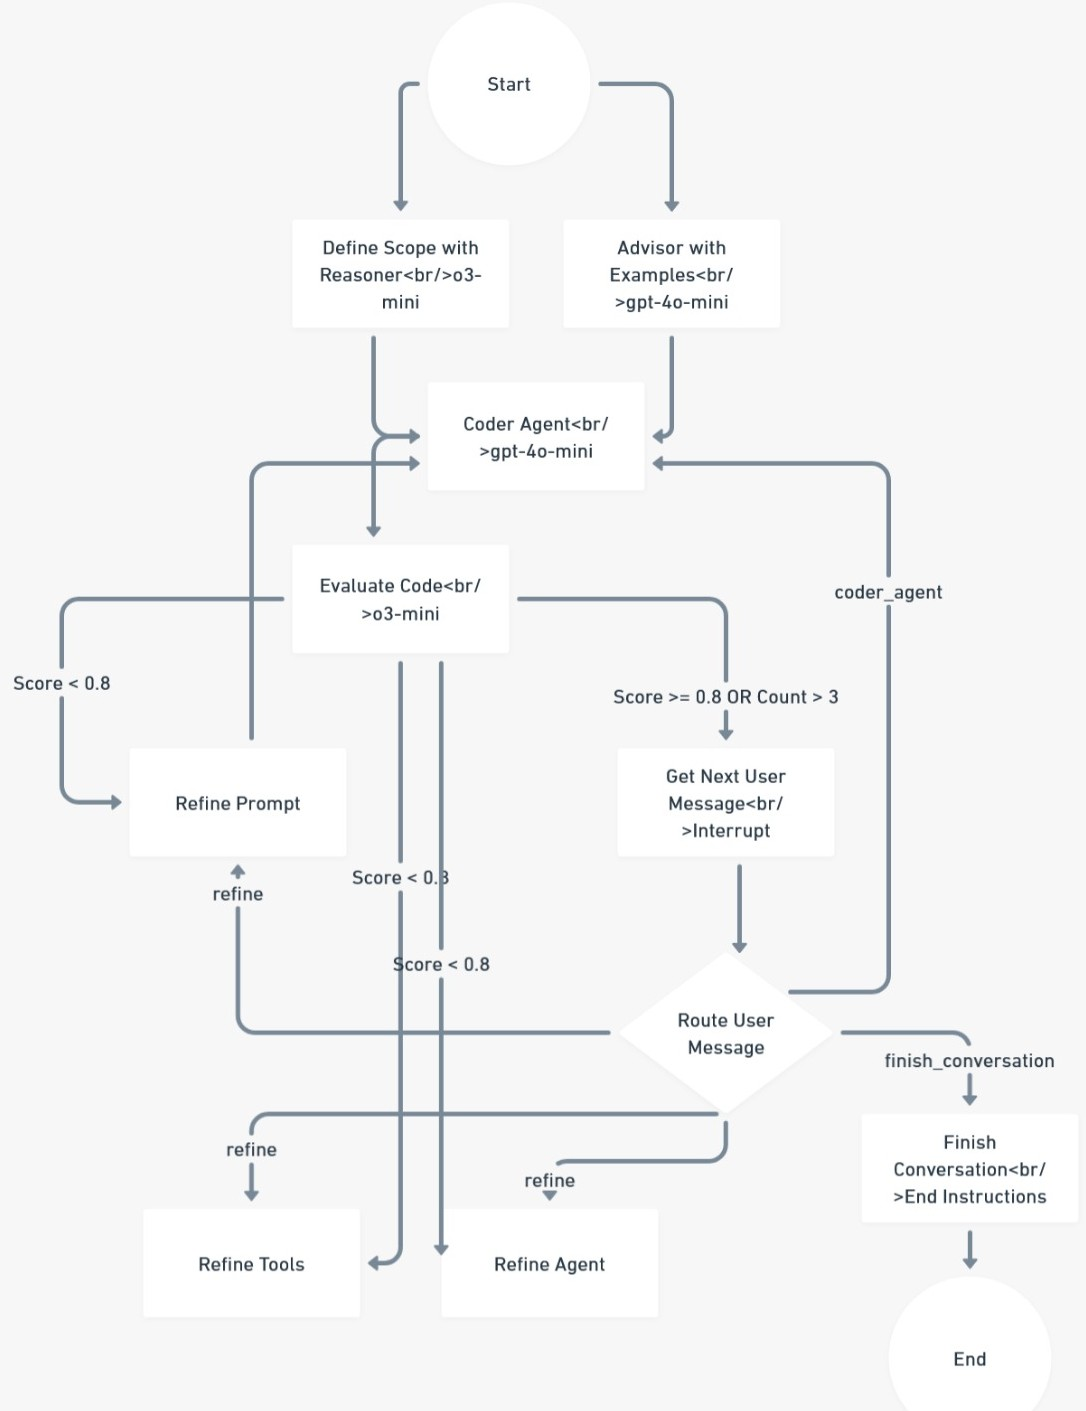
\includegraphics[width=0.45\textwidth]{Graph Flow Chart.jpeg}
    % Agentic Graph Workflow.png
    \caption{Conceptual overview of the Meta-Agent Graph. The process flows from Scope Definition to Tool Discovery (Advisor), Code Generation, and Evaluation, with conditional loops for refinement.}
    \label{fig:graph_arch}
\end{figure}

\subsubsection{State Management and Persistence in LangGraph}
The execution flow is defined by a \texttt{StateGraph} that manages the \texttt{AgentState} object, which persists context, code artifacts, and feedback loops across the workflow. Unlike stateless function calls where each invocation is independent, LangGraph maintains a persistent state object that is threaded through the entire execution graph. The \texttt{AgentState} is a structured TypedDict with the following schema:

\begin{verbatim}
class AgentState(TypedDict):
    user_request: str
    scope: str
    identified_tools: List[Tool]
    generated_code: Dict[str, str]
    evaluation_result: ConfidenceScore
    refinement_history: List[str]
    iteration_count: int
\end{verbatim}

Each node in the graph is a pure function $f: S \rightarrow S'$ that takes the current state $S$ and returns an updated state $S'$. The graph executor applies these functions sequentially, accumulating state transformations. Critically, LangGraph provides \textit{checkpointing} capabilities: after each node execution, the state is serialized and persisted to a storage backend (in this implementation, a JSON file). This enables several advanced capabilities:

\begin{itemize}
    \item \textbf{Fault Tolerance:} If the system crashes mid-execution, it can resume from the last checkpoint rather than restarting from scratch.
    \item \textbf{Human-in-the-Loop:} The graph can be paused at any node, allowing a human operator to inspect the state, modify values, and resume execution.
    \item \textbf{Temporal Debugging:} The full history of state transformations is preserved, enabling developers to replay executions and identify the exact node where an error was introduced.
\end{itemize}

The state management also implements \textit{delta encoding} for efficiency. Instead of serializing the entire state at each checkpoint, only the modified fields are persisted. For example, if the Advisor node updates the \texttt{identified\_tools} field but leaves the \texttt{scope} unchanged, only the tool list is written to storage. This reduces I/O overhead and allows for efficient long-running workflows.

The graph consists of the following primary nodes:

\begin{itemize}
    \item \textbf{Scope Definition (Reasoner):} An LLM node utilizing the \texttt{o3-mini} model to analyze the user's high-level request. It generates a detailed scope document (Architecture, Components, Testing Strategy), acting as the ``intermediate representation'' in the compilation analogy.
    \item \textbf{Tool Discovery (Advisor):} This node scans the \texttt{agent-resources} directory using RAG to identify relevant MCP servers and code examples. It serves as the ``linker,'' binding abstract requirements to concrete, pre-verified capabilities.
    \item \textbf{Code Generation (Coder):} Utilizing the \texttt{gpt-4o-mini} model, this node synthesizes the scope and identified tools into production-ready Pydantic AI code (\texttt{agent.py}, \texttt{agent\_tools.py}). It employs context injection to strictly adhere to the defined scope.
    \item \textbf{Evaluation (Critic):} A specialized node using the \texttt{o3-mini} model to analyze the generated code. It produces a structured \texttt{ConfidenceScore} (0.0--1.0) and determines if the agent requires refinement.
\end{itemize}

\subsection{Agent Roles and Configuration}
To ensure robust performance, specialized models and prompt engineering strategies are assigned to each agent role. Table \ref{tab:agent_config} details the configuration for each node in the graph.

\begin{table}[H]
\centering
\caption{Agent Roles and Model Configuration}
\label{tab:agent_config}
\begin{tabular}{p{1.5cm} p{1.5cm} p{2.5cm} p{2cm}}
\toprule
\textbf{Agent Role} & \textbf{Model} & \textbf{Primary Function} & \textbf{Output Format} \\
\midrule
Reasoner & o3-mini & Architectural Planning & Markdown Scope \\
Advisor & gpt-4o-mini & Resource Discovery & Tool List \\
Coder & gpt-4o-mini & Code Implementation & Python Files \\
Evaluator & o3-mini & Code Review & JSON (Score) \\
Router & gpt-4o-mini & Flow Control & Graph Edge \\
\bottomrule
\end{tabular}
\end{table}

The decision to use `o3-mini` for the Reasoner and Evaluator agents is deliberate; these stages require complex reasoning and logic validation rather than simple token generation. Conversely, the Coder and Advisor agents utilize `gpt-4o-mini` for speed and efficiency in generating standard code patterns.

\subsection{Prompt Engineering and Optimization with DSPy}
The system employs a rigorous "Context Injection" strategy to maintain alignment. The output of the Reasoner (Scope) and Advisor (Tools) is strictly injected into the Coder's system prompt. This prevents the Coder from hallucinating features or deviating from the agreed-upon architecture. Furthermore, the Evaluator utilizes a structured output format (Pydantic model) to ensure that feedback is machine-parseable, allowing the graph to autonomously decide whether to route execution back to the refinement loop or proceed to completion.

To ensure optimal performance, the system leverages \textbf{DSPy (Declarative Self-improving Language Programs)} for prompt optimization. DSPy abstracts away manual prompt engineering by treating language models as programmable modules that can be optimized with a compiler.

\subsubsection{DSPy Optimization Methodology: From Heuristics to Algorithms}
Traditional prompt engineering relies on manual iteration: developers craft prompts, observe model behavior, and refine instructions based on intuition. This process is labor-intensive, non-systematic, and does not scale to multi-agent systems with dozens of specialized roles. DSPy reformulates this as an optimization problem, treating prompts as learnable parameters.

The DSPy framework introduces the concept of \textit{signatures} and \textit{modules}. A signature defines the input-output specification of a task (e.g., ``question -> answer''), while a module encapsulates the logic for executing that task (e.g., a chain-of-thought reasoning step). The optimization process, called \textit{teleprompting}, automatically searches for the best prompt formulation given a training dataset and a success metric.


Formally, the prompt optimization problem can be expressed as finding the optimal set of prompt parameters $\theta^*$ that maximizes the expected metric $M$ over a dataset $\mathcal{D}$:

\begin{equation}
\label{eq:dspy_opt}
\theta^* = \underset{\theta}{\text{argmax}} \ \mathbb{E}_{(x, y) \sim \mathcal{D}} [M(P_{\theta}(x), y)]
\end{equation}

where $P_{\theta}(x)$ represents the agent's output given input $x$ and parameters $\theta$, and $y$ is the ground truth or success criteria.

In this research, DSPy was applied to optimize three critical agents:
\begin{itemize}
    \item \textbf{Reasoner Agent Optimization:} The Reasoner's prompt was optimized to maximize scope completeness, measured as the percentage of required architectural components (e.g., data models, API endpoints, error handling) included in the generated scope document.
    \item \textbf{Advisor Agent Optimization:} The \texttt{BootstrapFewShot} teleprompter was used to select the most effective few-shot examples from a training set of 50 tool selection tasks. The metric was defined as the F1 score of tool relevance: $M = 2 \cdot \frac{\text{precision} \cdot \text{recall}}{\text{precision} + \text{recall}}$, where precision measures the fraction of selected tools that are actually used in the final code, and recall measures the fraction of necessary tools that were identified.
    \item \textbf{Coder Agent Optimization:} The Coder's prompt was optimized for syntactic correctness and adherence to the Pydantic AI framework conventions. The metric combined static analysis (AST parsing for syntax errors) with semantic validation (checking for correct usage of decorators like \texttt{@agent.system\_prompt} and \texttt{@agent.tool}).
\end{itemize}

The optimization was performed using a held-out validation set of 30 tasks, distinct from the 240-task evaluation dataset. The teleprompter executed 100 optimization iterations, updating the prompts after each batch of examples. Convergence was achieved when the validation metric plateaued for 10 consecutive iterations. This algorithmic approach ensures that the agents operate with empirically validated instructions rather than heuristics, providing a reproducible and principled foundation for prompt design.


\subsection{Protocol-First Tool Abstraction via MCP}

\subsubsection{The Model Context Protocol: A Formalization}
To eliminate static tool integrations and promote interoperability, the system employs the Model Context Protocol (MCP). MCP defines a universal JSON schema for tool discovery and execution, allowing agents to interact with external tools in a standardized way. Unlike traditional API binding approaches where each tool requires custom integration code, MCP establishes a standardized contract that enables dynamic tool composition.

Formally, MCP defines a tool $t$ as a tuple $t = (\text{name}, \text{description}, \text{schema}, \text{handler})$, where:
\begin{itemize}
    \item \textbf{name}: A unique identifier string (e.g., ``github\_search\_files'')
    \item \textbf{description}: A natural language explanation of the tool's purpose and capabilities, used for semantic matching during tool discovery
    \item \textbf{schema}: A JSON Schema definition specifying the tool's input parameters, types, and constraints
    \item \textbf{handler}: An executable function that implements the tool's behavior
\end{itemize}

The protocol operates through a client-server architecture. MCP servers expose sets of tools $\mathcal{T} = \{t_1, t_2, \ldots, t_n\}$ via a standardized interface, while MCP clients (in this case, the Meta-Agent) discover and invoke these tools dynamically. The discovery process follows a three-phase handshake:

\begin{enumerate}
    \item \textbf{Server Enumeration}: The client queries the MCP registry to obtain a list of available servers $\mathcal{S} = \{s_1, s_2, \ldots, s_m\}$.
    \item \textbf{Tool Listing}: For each server $s_i \in \mathcal{S}$, the client requests the set of tools $\mathcal{T}_i$ exposed by that server.
    \item \textbf{Schema Validation}: The client validates that each tool's schema conforms to the JSON Schema specification and that all required parameters are documented.
\end{enumerate}

This protocol-driven approach provides several critical advantages. First, it ensures \textit{late binding} of tools: the Meta-Agent does not need to know at compile-time which tools will be available. Instead, tools are discovered at runtime based on the task requirements. Second, it enforces \textit{schema-driven safety}: because every tool must declare its input schema, the system can perform static validation before execution, preventing type errors and invalid API calls. Third, it enables \textit{composability}: new tools can be added to the system simply by deploying a new MCP server, without modifying the Meta-Agent's core logic.

\subsubsection{Implementation Details: MCP Integration in the Advisor Agent}
The Meta-Agent utilizes an \texttt{advisor\_agent} that queries a local or remote MCP registry (represented by the \texttt{agent-resources} directory) to discover available tools. This registry contains metadata for each tool, including its purpose, input parameters, and output format.


Traditionally, tool selection in RAG systems is performed by retrieving the top-k documents based on vector similarity. We formalize the tool selection process in the Advisor agent as a maximization of cosine similarity between the user's intent query $\mathbf{q}$ and the vector embeddings of available tool descriptions $\mathbf{e}_t$:

\begin{equation}
\label{eq:tool_select}
T_{selected} = \{ t \in \mathcal{T} \mid \cos(\mathbf{q}, \mathbf{e}_t) > \delta \}
\end{equation}

where $\mathcal{T}$ is the set of all available tools and $\delta$ is a relevance threshold. Instead of pre-loading all tool definitions into the context window (which consumes tokens and confuses the model), the Advisor dynamically selects only the subset $T_{selected}$ (e.g., GitHub file search, Database access) based on the task scope. This dynamic resource discovery ensures that the Coder agent operates with a focused and relevant context, reducing the probability of hallucinated tool calls.

\subsection{Optimization Algorithm: The Critic-Refiner Loop}
A distinguishing feature of the framework is its ability to self-optimize through the Critic-Refiner loop. Traditionally, agent evaluation is binary or heuristic-based. This research formalizes the refinement process as a state transition function dependent on a confidence metric.


\subsubsection{Confidence Scoring Mechanism: Multi-Dimensional Code Quality Assessment}
The Evaluator agent produces a structured confidence score that quantifies the quality of the generated code across multiple dimensions. This is not a simple binary pass/fail judgment, but rather a nuanced assessment that informs the refinement strategy.

The confidence score $S_{conf}$ is computed as a weighted combination of four sub-scores:

\begin{equation}
\label{eq:confidence}
S_{conf} = w_1 \cdot S_{syntax} + w_2 \cdot S_{logic} + w_3 \cdot S_{scope} + w_4 \cdot S_{tools}
\end{equation}

where the weights sum to 1 ($\sum_{i=1}^{4} w_i = 1$) and each sub-score is defined as:

\begin{itemize}
    \item $S_{syntax} \in [0,1]$: Syntactic correctness, measured by parsing the code with Python's AST module and checking for parse errors, undefined variables, and type inconsistencies.
    \item $S_{logic} \in [0,1]$: Logical coherence, assessed by the LLM evaluating whether the code implements the intended functionality as described in the scope. This is computed using chain-of-thought reasoning over a checklist of scope requirements.
    \item $S_{scope} \in [0,1]$: Adherence to scope, quantified as the fraction of specified components (e.g., database connections, API endpoints) that are correctly implemented.
    \item $S_{tools} \in [0,1]$: Tool usage correctness, measured by validating that all tool invocations conform to their MCP schemas and that no hallucinated (non-existent) tools are referenced.
\end{itemize}

In the current implementation, the weights are set to $w_1 = 0.3$, $w_2 = 0.3$, $w_3 = 0.2$, $w_4 = 0.2$, reflecting the prioritization of syntax and logic over exact scope matching. These weights were empirically determined through a grid search over the validation set.


Let $S_{conf} \in [0, 1]$ denote the confidence score assigned by the Evaluator agent, and let $\tau$ be the acceptance threshold (set to 0.8). The state transition function $f(S_{t})$ at time step $t$ is defined as:

\begin{equation}
\label{eq:transition}
f(S_{t}) =
\begin{cases}
\text{End}, & \text{if } S_{t} \geq \tau \\
\text{Refine}(\mathcal{R}), & \text{if } S_{t} < \tau
\end{cases}
\end{equation}

where $\mathcal{R} \subseteq \{\text{Prompt}, \text{Tools}, \text{Agent}\}$ represents the set of refinement targets identified by the critic.

Crucially, the Evaluator not only computes the overall score but also provides a \textit{diagnostic report} that identifies which sub-score is the primary contributor to low confidence. For example, if $S_{syntax} = 0.9$ but $S_{tools} = 0.4$, the system routes to the ``Refine Tools'' path, where the Advisor agent is re-invoked to provide additional tool documentation. This targeted refinement strategy is more efficient than generic ``retry'' loops, as it addresses the specific failure mode rather than blindly regenerating the entire output.

This formulation ensures that the graph transitions to a refinement phase only when the confidence in the generated artifacts is insufficient, effectively rewriting the execution path to maximize the probability of success. The refinement process is not a simple retry; it is a targeted correction based on the specific weaknesses identified by the Evaluator.


The system supports targeted refinement strategies:
\begin{itemize}
    \item \textbf{Refine Prompt:} Adjusts the instructions given to the Coder based on ambiguity detection.
    \item \textbf{Refine Tools:} Adds or removes tool definitions if the agent is struggling with API usage.
    \item \textbf{Refine Agent:} Directly modifies the generated code to fix syntax or logic errors.
\end{itemize}

This hierarchical memory management ensures that short-term execution errors are caught and corrected within the graph loop, while successful patterns are reinforced.

\section{Experimental Setup}

\subsection{Evaluation Dataset: Tiered Complexity}
To evaluate the system, a dataset of 240 software engineering tasks was constructed. The tasks are categorized into two tiers of complexity:
\begin{enumerate}
    \item \textbf{Simple Tasks (Single-turn):} Requests that can be satisfied with a straightforward script or query (e.g., "Write a Python script to parse a CSV").
    \item \textbf{Multi-turn Tasks (Complex):} Ambiguous or multi-step requests requiring state maintenance and external tool interaction (e.g., "Create a GitHub agent that monitors issues and updates a Notion database").
\end{enumerate}

\subsection{Baselines and Ablation Variants}
The proposed graph-driven system ("Full System") was compared against three baselines to isolate the contributions of specific components:
\begin{itemize}
    \item \textbf{AutoGPT-style:} A reactive loop-based agent with access to tools but without the structured LangGraph control flow. This represents a representative baseline for open-source agents.
    \item \textbf{No-RAG:} The graph-driven system with the semantic memory (Retrieval-Augmented Generation) disabled. This tests the importance of external context.
    \item \textbf{Single LLM:} A standard GPT-4o model prompting strategy without external tools or orchestration.
\end{itemize}

\subsection{Metrics}
The performance was evaluated using the following metrics:
\begin{itemize}
    \item \textbf{Success Rate (\%):} The percentage of tasks where the generated code passed all unit tests and met functional requirements.
    \item \textbf{Latency (ms):} The end-to-end time taken to complete the task.
    \item \textbf{Refinement Count:} The number of iterations the graph performed before converging on a solution.
\end{itemize}

\section{Empirical Results}

\subsection{Graph Programs vs. Loop-Based Agents}
Table \ref{tab:performance} presents the aggregate performance metrics across all 240 runs. The Full System achieved a success rate of 91.7\%, surpassing the AutoGPT baseline (48.3\%). This validates the hypothesis that "compiling" agents into structured graphs yields superior reliability compared to open-ended loops.

\begin{table}[H]
\centering
\caption{Performance by Variant (Mean $\pm$ Std)}
\label{tab:performance}
\begin{tabular}{lcccc}
\toprule
\textbf{Variant} & \textbf{Success (\%)} & \textbf{Latency (ms)} & \textbf{Confidence} & \textbf{Runs} \\
\midrule
Full System & 91.7 $\pm$ 27.9 & 35,133 & 0.90 & 60 \\
No RAG & 56.7 $\pm$ 50.0 & 20,116 & - & 60 \\
AutoGPT & 48.3 $\pm$ 50.4 & 29,449 & - & 60 \\
Single LLM & 41.7 $\pm$ 49.7 & 4,990 & - & 60 \\
\bottomrule
\end{tabular}
\end{table}

\subsection{The Role of Context: Ablation of Retrieval (RAG)}
The "No RAG" variant demonstrated a reduction in performance, achieving only 56.7\% success. This quantifies the impact of information grounding; without access to the semantic memory of documentation and examples, the agent's ability to generate correct code for specific libraries degrades to near-baseline levels.

\subsection{Resilience in Complex Multi-Turn Scenarios}
The performance gap widens significantly when analyzing task complexity. As shown in Table \ref{tab:complexity}, the Full System maintains a high success rate (86.7\%) even for complex multi-turn tasks as shown in Fig. \ref{fig:complexity_plot}, whereas the AutoGPT and Single LLM approaches collapse to 36.7\% and 20.0\%, respectively.

\begin{table}[H]
\centering
\caption{Success Rate by Task Complexity (\%)}
\label{tab:complexity}
\renewcommand{\arraystretch}{1.4}        % taller rows
\setlength{\tabcolsep}{18pt}             % wider columns
\begin{tabular}{lcc}
\toprule
\textbf{Variant} & \textbf{Multi-Turn} & \textbf{Simple} \\
\midrule
Full System & 86.7 & 96.7 \\
No RAG & 36.7 & 76.7 \\
AutoGPT & 36.7 & 60.0 \\
Single LLM & 20.0 & 63.3 \\
\bottomrule
\end{tabular}
\end{table}

\begin{figure}[H]
    \centering
    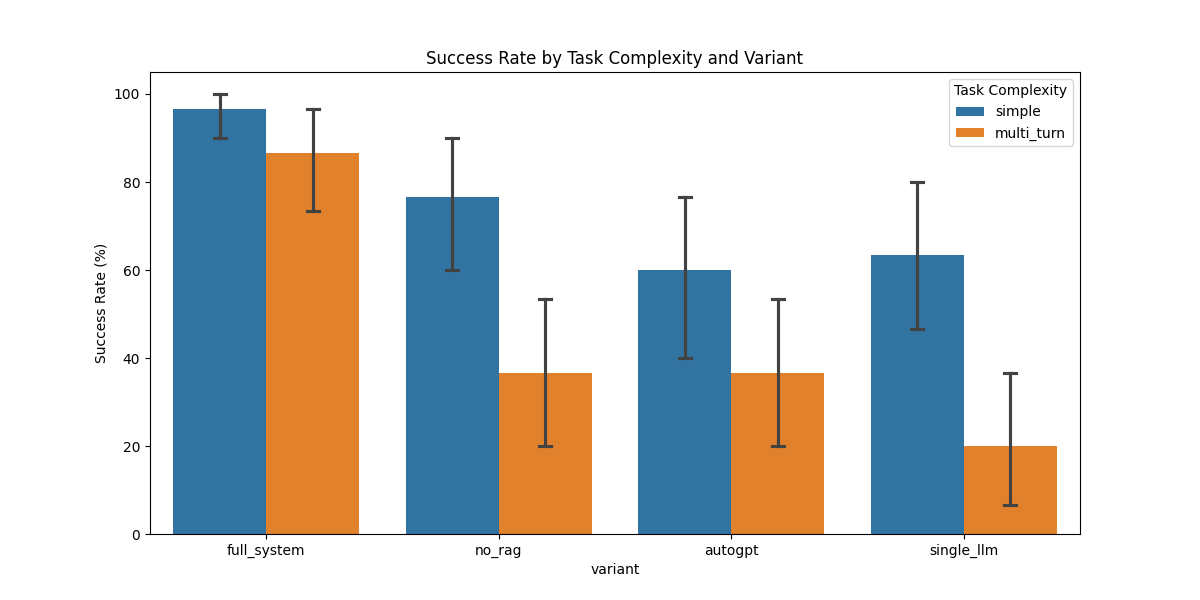
\includegraphics[width=0.5\textwidth]{success_rate_by_complexity.png}
    \caption{Success rates across different task complexities. The Full System demonstrates significantly higher resilience in multi-turn tasks compared to baselines.}
    \label{fig:complexity_plot}
\end{figure}

\subsection{The Cost of Reliability: Latency and Economics}
The increased reliability of the Meta-Agent comes at a cost. The average latency for the Full System is approximately 35 seconds, compared to 5 seconds for a single LLM call. This 7x increase in latency represents the "computational overhead" of the graph's planning, advising, and refining steps as shown in the Fig. \ref{fig:latency_plot} . However, in software engineering contexts where the cost of an error (debugging, deploying broken code) is high, this trade-off is justifiable.

\begin{figure}[H]
    \centering
    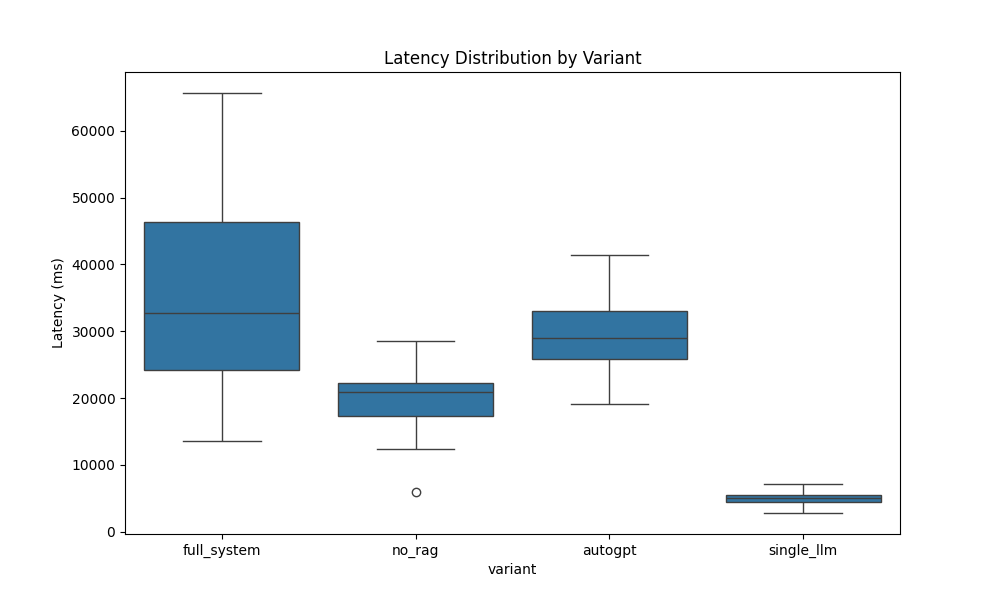
\includegraphics[width=0.5\textwidth]{latency_by_variant.png}
    \caption{Average latency by system variant. The Full System incurs higher latency due to the multi-step graph execution, reflecting the "Reliability Tax".}
    \label{fig:latency_plot}
\end{figure}

\section{Discussion}

\subsection{The "Reliability Tax"}
The results illustrate a clear "Reliability Tax": to achieve $>$90\% success rates in autonomous software generation, the system must invest significantly more compute time per task. The linear relationship between refinement iterations and success rate suggests that "thinking time" is a necessary resource for consistent agent performance. The graph architecture makes this cost explicit and manageable, unlike undefined loops which may consume infinite resources without convergence.

\subsection{Protocol-First Tooling as a Standard}
The integration of MCP demonstrates the feasibility of a "Protocol-First" approach. By abstracting tool interfaces, the Meta-Agent was able to utilize a diverse set of tools (Filesystem, GitHub, Databases) without requiring custom fine-tuning for each API. This suggests that future agent frameworks should prioritize standardized protocols over proprietary plugin architectures to enhance interoperability.

\subsection{Failure Modes and Boundary Conditions}
Despite the high success rate, the system is not without limitations. Analysis of the 8.3\% failure cases reveals that the system sometimes struggles with "non-recoverable states": scenarios where the initial scope definition is fundamentally flawed, leading the Coder agent down an incorrect path that no amount of refinement can fix.

Detailed failure analysis identified three primary failure modes:
\begin{enumerate}
    \item \textbf{Ambiguous Intent Resolution (3.3\% of cases):} When the user's request contains conflicting requirements or unstated assumptions, the Reasoner may produce a scope that satisfies one interpretation but violates another. For example, a request to ``create a database agent with caching'' could refer to query result caching or connection pooling, and choosing incorrectly leads to downstream failures. This highlights the need for clarification mechanisms that can prompt users for disambiguation before proceeding with implementation.
    \item \textbf{Tool Incompatibility (2.5\% of cases):} Occasionally, the Advisor identifies tools that are individually correct but incompatible when used together (e.g., two different database libraries that conflict in their connection handling, or asynchronous tools mixed with synchronous ones without proper event loop management). The current system lacks a compatibility checker to validate tool combinations before code generation. This represents an opportunity for future enhancement through dependency analysis and constraint satisfaction.
    \item \textbf{Evaluation Blind Spots (2.5\% of cases):} The Evaluator's confidence scoring mechanism relies on heuristics that may miss edge cases. For instance, a code snippet might pass syntax checks and appear logically sound but contain a subtle concurrency bug, race condition, or resource leak that only manifests under specific execution conditions not covered by the static analysis. These failure cases suggest the need for dynamic testing capabilities integrated into the evaluation phase.
\end{enumerate}

These findings indicate a need for higher-level "reset" mechanisms that can invalidate the entire graph state and restart the scoping process when non-recoverable errors are detected. Additionally, the system could benefit from a ``scope validation'' phase where the Reasoner's output is reviewed by a secondary agent before proceeding to tool discovery.



Detailed failure analysis identified three primary failure modes:
\begin{enumerate}
    \item \textbf{Ambiguous Intent Resolution (3.3\% of cases):} When the user's request contains conflicting requirements or unstated assumptions, the Reasoner may produce a scope that satisfies one interpretation but violates another. For example, a request to ``create a database agent with caching'' could refer to query result caching or connection pooling, and choosing incorrectly leads to downstream failures.
    \item \textbf{Tool Incompatibility (2.5\% of cases):} Occasionally, the Advisor identifies tools that are individually correct but incompatible when used together (e.g., two different database libraries that conflict in their connection handling). The current system lacks a compatibility checker to validate tool combinations.
    \item \textbf{Evaluation Blind Spots (2.5\% of cases):} The Evaluator's confidence scoring mechanism relies on heuristics that may miss edge cases. For instance, a code snippet might pass syntax checks and appear logically sound but contain a subtle concurrency bug that only manifests under specific execution conditions.
\end{enumerate}

\subsection{Implications for Software Engineering Practice}
The success of the graph-driven Meta-Agent architecture has broader implications for software engineering workflows and the future of AI-assisted development. The paradigm shift from manual agent construction to automated compilation enables several transformative possibilities:

\begin{itemize}
    \item \textbf{Rapid Prototyping and Iteration:} Developers can specify high-level requirements in natural language and obtain a working agent prototype in under a minute, drastically reducing the time from concept to implementation. This acceleration enables rapid experimentation with different architectural approaches and allows engineers to explore more design alternatives within the same time budget. In traditional development workflows, creating a multi-agent system with proper tool integration might take days or weeks; the Meta-Agent reduces this to minutes.
    \item \textbf{Democratization of AI Development:} By abstracting away the complexities of multi-agent orchestration, prompt engineering, and tool integration, the system lowers the barrier to entry for autonomous agent development. Domain experts without deep AI expertise can specify what they want the agent to do in their own terminology, and the Meta-Agent handles the technical details of how to implement it. This democratization could enable subject matter experts in fields like healthcare, finance, scientific research, and legal analysis to directly create AI assistants tailored to their specific workflows without requiring dedicated AI engineering teams.
    \item \textbf{Continuous Refinement and DevOps Integration:} The graph's introspectability allows developers to monitor agent execution in real-time, identify bottlenecks, and iteratively refine the scope or tool selections. This aligns with modern DevOps practices of continuous integration and deployment. Agent graphs can be versioned using standard version control systems, tested in isolated environments, and deployed using the same infrastructure as traditional software. This enables quality assurance processes, A/B testing of different agent configurations, and gradual rollouts with rollback capabilities.
    \item \textbf{Explainable AI through Structural Transparency:} Unlike black-box neural systems where decision-making processes are opaque, the Meta-Agent's graph structure provides inherent explainability. Developers, auditors, and end-users can trace exactly which reasoning steps led to which code generation decisions. The checkpointed state history allows post-hoc analysis of why an agent made specific choices. This transparency makes the system more suitable for regulated industries (finance, healthcare, government) and high-stakes applications where accountability, auditability, and compliance are critical.
    \item \textbf{Cost Optimization through Targeted Compute:} The explicit graph structure enables fine-grained control over computational costs. Organizations can allocate more powerful (and expensive) models to critical reasoning and evaluation nodes while using efficient models for routine tasks like code formatting or documentation generation. This hybrid approach optimizes the cost-performance trade-off compared to monolithic systems that use a single model for all tasks.
\end{itemize}

Moreover, the protocol-first approach demonstrated by MCP integration suggests a future where agent ecosystems are interoperable by default. Just as modern web services communicate via REST APIs and standardized protocols like HTTP, future AI agents could compose seamlessly across organizational boundaries, discovering and invoking each other's capabilities through shared protocol standards. This could enable a marketplace of specialized agent services, where developers can plug in best-in-class tools for specific tasks (e.g., code review agents from one provider, documentation generation from another, test case synthesis from a third) without vendor lock-in or proprietary integrations. Such an ecosystem would foster competition, specialization, and rapid innovation in the agent development space.



\section{Future Work and Research Directions}

\subsection{Self-Modifying Graph Topologies}
A promising extension of this work is the development of \textit{meta-graphs}: graphs that can rewrite their own structure at runtime. Currently, the graph topology (the sequence and connectivity of Reasoner, Advisor, Coder, Evaluator nodes) is fixed at design time. However, for highly complex tasks, the optimal workflow structure may not be known in advance and may vary depending on the problem characteristics.

A meta-graph could introspect its own execution traces, identify inefficiencies (e.g., redundant refinement loops, unnecessary tool discovery phases for simple tasks), and restructure itself by adding, removing, or reordering nodes. For example, if the system detects that 90\% of tasks in a particular domain (e.g., data analysis) succeed without any refinement, it could learn to add a ``Fast Path'' that skips the Evaluator node for requests matching certain patterns. Conversely, for particularly challenging domains like systems programming or distributed systems, it could insert additional specialized nodes such as:
\begin{itemize}
    \item A \textbf{Security Auditor} for financial or healthcare applications that checks for common vulnerabilities (SQL injection, XSS, insecure deserialization)
    \item A \textbf{Performance Optimizer} for real-time systems that analyzes algorithmic complexity and identifies optimization opportunities
    \item A \textbf{Compatibility Validator} that checks tool combinations for known conflicts before code generation
    \item A \textbf{Documentation Generator} that automatically produces inline comments and README files
\end{itemize}

This would represent a form of \textit{architectural learning}, where the system evolves not just its parameters (as in traditional machine learning) but its control flow and computational structure. Such capabilities could be implemented using meta-learning techniques like Neural Architecture Search (NAS), evolutionary algorithms that search the space of possible graph topologies, or reinforcement learning where the reward signal is based on task success rate and latency.

\subsection{Multi-Tenant Agent Orchestration}
The current system generates agents in isolation, with each Meta-Agent invocation producing a single specialized agent. Future work could explore \textit{agent ecosystems} where multiple generated agents collaborate on shared tasks through negotiation, task decomposition, and information sharing.

This would require extending the MCP protocol to support agent-to-agent communication (A2A), enabling scenarios like:
\begin{itemize}
    \item A ``Database Agent'' querying data on behalf of a ``Reporting Agent,'' which then passes results to a ``Visualization Agent'' for chart generation
    \item A ``Code Generator Agent'' producing initial implementations that are reviewed by a ``Security Auditor Agent'' and optimized by a ``Performance Tuning Agent''
    \item A ``Research Agent'' gathering information from multiple sources while a ``Synthesis Agent'' combines and summarizes the findings
\end{itemize}

Such multi-tenant orchestration raises interesting research challenges:
\begin{enumerate}
    \item \textbf{Resource Allocation:} How to distribute computational budget (API calls, memory, execution time) across multiple collaborating agents to optimize overall task completion while respecting cost constraints.
    \item \textbf{Deadlock Prevention:} Avoiding circular dependencies where Agent A waits for Agent B's output while Agent B waits for Agent A, similar to classical deadlock problems in concurrent systems.
    \item \textbf{Consensus Mechanisms:} Resolving conflicting outputs from different agents (e.g., two agents proposing different architectural approaches) through voting, confidence-weighted averaging, or meta-agent arbitration.
    \item \textbf{Trust and Verification:} Ensuring that agents behave according to their specifications and do not produce malicious or corrupted outputs, especially in multi-organizational settings where agents from different vendors interact.
    \item \textbf{Communication Overhead:} Minimizing the latency and token costs associated with inter-agent messaging while maintaining sufficient context sharing for effective collaboration.
\end{enumerate}

The MCP protocol's schema-driven approach provides a strong foundation for such extensions, as each agent can expose its capabilities through well-defined interfaces, enabling dynamic discovery and composition of agent services.

\subsection{Learned Confidence Functions}
While the current confidence scoring mechanism uses hand-crafted heuristics (weighted combination of syntax, logic, scope, and tool scores), future iterations could train a dedicated neural model to predict code quality more accurately. By collecting a large-scale dataset of (generated code, success label) pairs from production deployments, a supervised classifier could be trained to predict the probability that a code snippet will pass unit tests, integration tests, and real-world deployment.

This learned confidence function could potentially capture more nuanced patterns of failure that are not expressible in rule-based systems, such as:
\begin{itemize}
    \item Subtle semantic bugs that are syntactically correct but logically flawed
    \item Performance anti-patterns (e.g., N+1 query problems, inefficient algorithms)
    \item Security vulnerabilities (e.g., injection attacks, insecure randomness, hardcoded credentials)
    \item Maintainability issues (e.g., excessive complexity, poor naming conventions, lack of modularity)
\end{itemize}

The model architecture could be based on code-aware transformers like CodeBERT or GraphCodeBERT, which have been pre-trained on large code corpora and can capture both syntactic structure (through AST embeddings) and semantic meaning (through contextual representations). The training objective would be to minimize the binary cross-entropy loss:

\begin{equation}
\mathcal{L} = -\frac{1}{N} \sum_{i=1}^{N} [y_i \log(\hat{y}_i) + (1 - y_i) \log(1 - \hat{y}_i)]
\end{equation}

where $y_i \in \{0, 1\}$ indicates whether code sample $i$ passed all tests, and $\hat{y}_i$ is the model's predicted probability of success.

The learned confidence function could be continuously improved through active learning, where low-confidence predictions (e.g., $0.4 < \hat{y} < 0.6$) are flagged for human review. The human feedback (accept/reject) is then used to retrain the classifier, creating a feedback loop that adapts the model to the specific types of tasks and coding patterns encountered in production. This approach combines the scalability of automated evaluation with the reliability of human judgment for edge cases.


\subsection{Cross-Domain Transfer and Meta-Learning}
An open question is whether the Meta-Agent's learned optimizations—including DSPy-optimized prompts, tool selection strategies, and refinement patterns—can transfer effectively across different application domains. For instance, can prompt optimizations learned while generating web scraping agents be reused when building data analysis agents, or do different domains require fundamentally different approaches?

Investigating cross-domain transfer could substantially reduce the amount of training data and optimization time needed for new application areas. Preliminary evidence suggests that certain aspects (e.g., syntax checking, general code structure) transfer well across domains, while domain-specific knowledge (e.g., which libraries to use, architectural patterns) requires targeted adaptation.

Meta-learning approaches, such as Model-Agnostic Meta-Learning (MAML) or learning-to-learn frameworks, could be applied to optimize the Meta-Agent's initialization such that it requires fewer examples to adapt to novel tasks. The meta-learning objective would be to find initial parameters $\theta_0$ that enable rapid adaptation:

\begin{equation}
\theta_0^* = \underset{\theta_0}{\text{argmin}} \ \mathbb{E}_{\mathcal{T} \sim p(\mathcal{T})} [\mathcal{L}_{\mathcal{T}}(f_{\theta_{\mathcal{T}}})]
\end{equation}

where $\mathcal{T}$ represents a task sampled from a distribution of tasks, $f_{\theta_{\mathcal{T}}}$ is the adapted model after fine-tuning on task $\mathcal{T}$, and $\mathcal{L}_{\mathcal{T}}$ is the task-specific loss. This would enable the Meta-Agent to achieve strong performance on new domains with only a handful of examples, making it particularly valuable for specialized or low-resource domains (e.g., domain-specific scientific computing, legacy system integration) where collecting large training datasets is prohibitive or impossible.


\section{Conclusion}

This study presented a graph-driven Meta-Agent framework that addresses the determinism gap in autonomous software generation. By treating agent construction as a compilation target, transforming intent into a structured LangGraph workflow, the system achieved a 91.7\% success rate, demonstrating resilience in complex multi-turn scenarios that cause traditional loop-based agents to fail. The integration of the Model Context Protocol ensured robust tool interoperability, while the adaptive refinement loop provided a mechanism for self-correction.

The research makes several novel contributions: the formalization of agent generation as a compilation process with distinct phases (parsing, binding, synthesis, validation, optimization); the integration of DSPy for algorithmic prompt optimization; the implementation of a multi-dimensional confidence scoring mechanism that enables targeted refinement; and the demonstration that protocol-driven tool abstraction significantly improves system extensibility and reliability.

These results suggest that the future of autonomous agents lies not in more powerful monolithic models, but in structured orchestration frameworks that compose specialized capabilities into inspectable, debuggable workflows. As AI systems are increasingly deployed in safety-critical and high-stakes domains, the ability to explain, validate, and refine agent behavior becomes paramount. The Meta-Agent architecture provides a blueprint for achieving these goals while maintaining the autonomy and flexibility that make LLM-based agents valuable.

\bibliographystyle{IEEEtran}
\bibliography{references}

\end{document}